\section{Attacks}

%\subsection{Exploiting Condition}
%\paragraph{App Description}
%\paragraph{Timer}

\subsection{Threat Model}
Our analysis is built on arbitrary Android device environment with an adversary app stealthily running on the background out of user's awareness.  The adversary needs to conceal its behaviours and minimize its impact on the device performance. The goal of attackers is to conduct the \emph{event hijacking} exploiting certain victim app and to achieve its malicious purpose(e.g., obtain user's sensitive data and escalate access privilege). The adversary app is supposed to be installed without requesting any permissions except several common-used permissions like INTERNENT, which is commonly required by existing attacks on Android OS\cite{chen2014peeking}\cite{ren2015towards}. In some special scenarios, insensitive permissions for users such as BATTERY\_STATS are also allowed to be requested to predict victim's related \emph{control confidentiality}. 


%The adversary is supposed having the capability of using public  and analysing them on the fly. Again, . As introduced in "Callback State Model", this capability can be obtained by particular methods within ActivityManager class.
%it should stay aware of the running states of apps and some particular services
\subsection{Attacks Exploiting the PEC Threats}

\begin{figure}
\centering
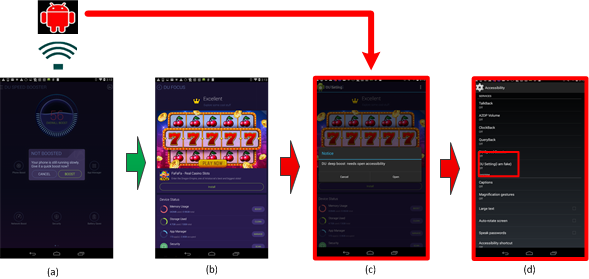
\includegraphics[width = 3.0in]{pic2.png}
\caption{\label{}Example of Dialog Escalation with PEC threats}
\end{figure}

\begin{figure}
\centering
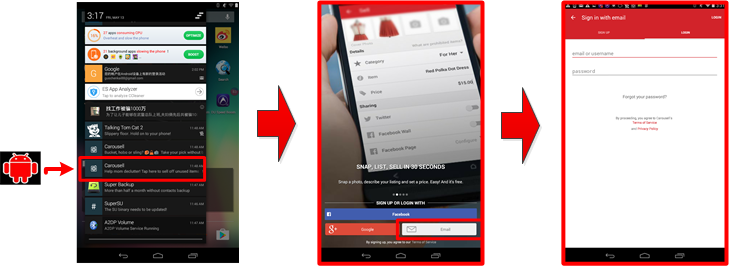
\includegraphics[width = 3.0in]{pic3.png}
\caption{\label{}Example of Notification Forgery with PEC threats}
\end{figure}

\begin{figure}
\centering
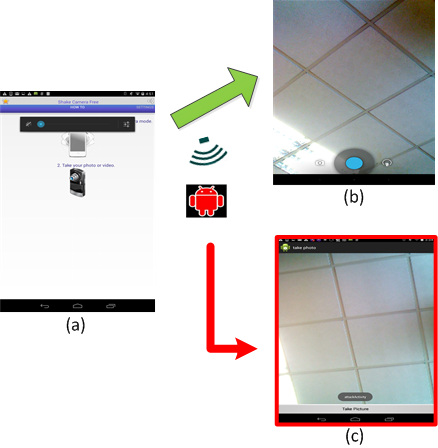
\includegraphics[width = 3.0in]{pic4.png}
\caption{\label{}Example of Shaking Spoofing with PEC threats}
\end{figure}

\begin{figure}
\centering
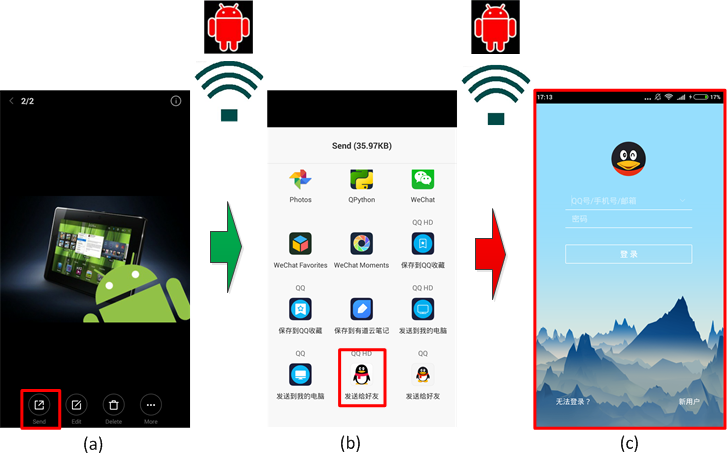
\includegraphics[width = 3.0in]{pic5.png}
\caption{\label{}Example of Activity Phishing with PEC threats}
\end{figure}

In order to understand the attack feasibility of PEC threats, we explore typical types of attacks and present a detailed description of them in this section. Here, we represent one type of attack aiming to each display-sink as a fundamental exploration effort. We can foresee more attack types will continually emerge once the PEC threats are commonly noticed by attackers. 

%Following represents typical attacks forms that utilizes the PEC of victim app or PEC itself. According to the display-sink a PEC ends to, we representatively list several main types of attack examples, namely dialog \& toast privilege escalation, notification forgery, shaking-display spoofing and activity phishing. 
\subsubsection{Dialog \& Toast Privilege Escalation}

%A typical implementation of above logic is represented as following:
%\begin{figure}
%\centering
%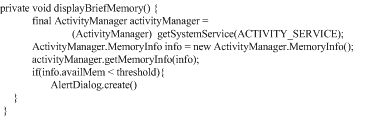
\includegraphics[width = 3.0in]{code1.png}
%\caption{\label{}control-flow}
%\end{figure}

Both of Dialog and Toast(D\&T for short) act as a type of window display for notifying users the intermediate results or alert information when a particular event happens. Previous attacks haven't pay enough attention to Dialog and Toast since the size of information carried by them is too small to make considerable security impact. Most of existing attacks upon D\&T rely on fooling user by a lure surface, which emerges in a sudden way that inevitably arises user's suspicion. In contrast, exploiting PEC threats is able to control the attack timing in reasonable scenes.

\textbf{PEC analysis.} %Once a public event is received, an adversary app would be easy to predict the time when a dialog or toast really emerges as long as the targeted app lacks of complex condition constrains in its control flow of the key callbacks. 
Compared to sensitive information, D\&T are more likely to reflect real-time status about either app execution or system relevant resources such as \textit{battery}, \textit{memory}, \textit{voice}, etc. However, most of these statuses are closely connected to PE trigger (e.g., system will send BATTERY\_LOW event to indicate low battery condition on the device, which can be received by ordinary apps). Therefore, a PEC threat contained by the D\&T or Toast holder  provides an indirect way for attacker understanding the popping up timing of certain D\&T and Toast. Further, attackers can employ user's trust of such D\&T holder to get the same trust for their adversaries.

System management apps(e.g., DU Speed Booster, Avast Cleanup, etc.) can be treated as a typical type of such D\&T holder since they need to frequently prompt user about system running status. Here, we take the storage status as an illustration example. When the free storage of system rests as low as a given level, a DEVICE\_STORAGE\_LOW event serves as a public event and will be sent out by system itself. Professional system management apps installed on the device receive the event by background \textit{Service} that drives a \textit{BroadcastReceiver}. The receiver PEC \texttt{onRecevie()} of the BroadcastReceiver filters the received public event. If the receiver PEC links to a D\&T display window (e.g., pop up a corresponding Dialog with a short alarm message \textit{"Your phone is still running slowly. Give it a deep boost now?"}), the D\&T can be predicted to be popped up on foreground in seconds. The PEC threats here assists to expose the certain knowledge about running stage (\textit{"Hey! I have prepared to release the occupied storage!"}) of such system management apps.

%and request user's decision whether to release the wasted occupation. If user  agree button, a new process launched by the manager app starts running.

%these kinds of notices are sent by pre-installed or system manager apps. Also, users are with fully trust for these apps in security part because they are professional and have numerous of users. However, this trust acts as a big opportunity that can be exploited to achieve the attack goal in attacker's eyes.

%The key point is the memory status(info.availMem) are public resources and can be obtained by any app installed in the device without any permission request. Moreover, the implementation control flow is designed so simple that 
%the condition logic and variable "threshold" could be easily reconstructed in an adversary app. A experienced attacker could also obtain the these key logic and variables through reverse-engineering and binary analysis. As a result, the condition "info.availMem < threshold" as a public events makes the function "AlertDialog.create()" a PEC, and attackers are able to judge the creating time of the AlerDialog from its own reconstructed adversary app installed in the same device.

\textbf{Attack Implementation.}
The analysed exposure scenario offers attacker opportunities to construct attacks escaping user's awareness. We take a privilege escalation as an illustration attack example. Figure * presents such an attack procedure for an attacker getting the \textit{Accessibility Service} grant from user. The \textit{Accessibility Service} serves as a specific functionality supplied by Android to help disabled people conveniently obtain the component status and handle the device operations . Android supports richer interfaces of the \textit{Accessibility Service} after 4.0 version, which on the other side arises higher security risk. Hence, it is restricted by Android that all relevant implementations have to be engaged under the user's manual grant in the setting option page.

% for developers implementing their Accessibility functionalities like listening user actions. Undoubtedly, this functionality is so powerful that it is impossible to be ignored by attackers. However,  It seems infeasible for attackers to get the grant directly. After all, it performs very suspicious if such a setting window suddenly opens on the foreground against user's intention.
If an advarsary app desires to obtain the \textit{Accessibility Service} grant, it is infeasible to pop up the grant page in an improper scenario causing an unreasonable display can easily arise user's suspicion. However, by exploiting the PEC of such a trusted system management app, the attack procedure could become more reasonable to escape user's perceptiveness. 

The background adversary service first monitors if the PEC service is running through the \texttt{getRunningServices()} offered by the \texttt{ActivityManager}. Fortunately, the invoking of \texttt{getRunningServices()} needs not any permission request and has not been constrained as the \texttt{getRunningTasks()}(mentioned in Section *) so far. 

After that, the adversary waits for the PE (the free memory size falls below a given threshold) coming using the same logic designed by trusted victim app. Once the PE happens, the adversary understands that the victim has prepared to release storage (Figure *(a)). At this point, adversary shows its own fake Dialog covering on the original one, avoiding user seeing it (Figure *(c)). In the fake Dialog, a lure message tells user a corresponding \textit{Accessibility Service} have to be grant to complete the cleaning storage task. Once user clicks \textit{Agree} button, a \textit{Accessibility Service} setting page is automatically opened on the foreground using Setting.ACTION\_ACCESSIBILITY\_SETTINGS intent as Figure *(d) did. For further conceal the attack feature, the name of malicious \textit{Accessibility Service} is camouflaged as the confused one (e.g., "DU deep boost" for forging the \textit{DU booster} app ). In practice, we take 2s delay for catering the emergence of targeted Dialog. 

\subsubsection{Notification Forgery}
The Notification in Android normally works for showing the received updated message and the task progress information, which is somehow similar as D\&T. Different from the latter, the user is not necessary to immediately handle the message sent by a Notification. Instead, the developer uses \texttt{PendingIntent} to handle intent in the future, which is upon when user clicks the Notification. 

 %in the Notification Drawer

%Again, a Notification would not disappear in seconds as the Toast does until user handles it. The user could handle it at any time they like, which gives attackers enough time to forge a fake one escaping user's attention. Here we introduce two common used situations. 

\textbf{PEC analysis.}
Most of the market apps currently are based on CS (Client-Server) pattern, and the server needs to frequently push the updating data to the client (app installed in user's device). The client keeps running a service in the background to communicate with the server. Normally, this push-receive mechanism is implemented by specialized module with high-level security protection that makes it hard to get any push status by other apps. However, since the status of client service is publicly opened, adversary also could exploit it to fool the user in an indirect way. 

First, through pre-analysing the service of victim app for handling the pushed data, an attacker can judge whether it's PECs links to a Notification display or not. If the life-cycle PEC onCreate() indeed links to a Notification sending logic, the adversary can receive a signal from the victim service that it keeps receiving the pushed data and sending Notification. Given that knowledge, the adversary judges that a same Notification sending action is hard to arise user's suspicion.   

%Besides that, another PEC threat emerges when the user clicks on the Notification. There are two PEs within this process. One is the change of the Notification Drawer serves as the PE, causing other apps can deceive it through the open APIs provided by \texttt{NotificationManager} without permission request.

\textbf{Attack Implementation.}
Consider the app Carousell, a popular goods-trading platform that frequently sends Notification notifying it's new selling information to user. Normally, Carousell builds a resident service \texttt{PendingIntentCallbackService} running on the background. When an adversary observes it's running, a fake Notification constructed with the same resources and framework as original Carousell did(Figure * (a)). Fortunately, Android system currently allows a developer to arbitrarily build the appearance of its own Notification, especially the icon and content. The relevant open APIs are provided in the \texttt{Builder} class (e.g., \texttt{setContentTitle()}, \texttt{setContentText()}, \texttt{setSmallIcon()}, etc.). Different with the benign Notification, the fake one is connected to a carefully constructed \textit{Carousell login} page that needs user input their Carousell account(even the account of third-party single sign-on Facebook and Google)(Figure * (b)\&(c)). When the user opens the Notification Drawer, there are several very similar Notifications listing there(as Figure * (a) shows). If the user chooses the fake one and tries to log in the Carousell account, the user name and password will be delivered to the attacker through network.


%\# Notice. Another important usage of the Notification is to notify users update status from a specific app or the device system. For instance, the QPtyhon(An app for python debugging on Android) would perform a log Notification when the onDestroy() lifecycle function in the MainActivity happens. However, since the onDestroy() is invoked when the MainActivity is destroyed, a third-party app uses the getRunningAppProcesses()(offered by ActivityManager) function to judge it. Thus, the onDestroy() belongs to the PEC as well. Attackers could capture the time of such Notification emergence and even the time user triggers the Notification(when the targeted Notification is dismissed and corresponding app starts running.)by analysis from getActiveNotifications() offered by NotificationManager(after Android 4.3) 

%Once it happens, the adversary would predict the notice Dialog will pop up in a few seconds(Figure *(a)).

% After that, it shows a Dialog tip(Figure *(c)) to tell user the corresponding Accessibility Service have to be grant to complete the data clean task, and then opens the Accessibility Service setting page using "Setting.ACTION\_ACCESSIBILITY\_SETTINGS" intent like Figure *(d) did. In the setting page, an attack service with a confused name "DU deep boost" fool user about this attack. At last, the adversary app gets the grant and could engage further attacks. 



%In order to clearly illustrate the attack process, first the threat model need to be depicted.
%Suppose that we have a victim app installed in a given device, and it contains corresponding callback threats vulnerabilities. Besides, suppose that we have an adversary app installed in the same device and start its service running on the background stealthily. The goal of our adversary app is to engage diverse attacks through the victim app. In theory, the adversary app need not apply any permission when it is installed. However, in practice, it needs to apply some  common-used permissions like "Internet" and insensitive permissions like "batter related permission" according to the attack type. The adversary needs to visually conceal its behaviours from users and also minimize its impact on the device performance. 

%The adversary is supposed having the capability of using public available resources and analysing them on the fly. Again, it should stay aware of the running states of apps and some particular services. As introduced in "Callback State Model", this capability can be obtained by particular methods within ActivityManager class.

%\section{Attacking PEC Weakness}

%\subsection{Exploiting Condition}
%\paragraph{App Description}
%\paragraph{Timer}

In this section, we present several concrete attacks against real-world apps which have the PEC weakness. 
These attacks demonstrate that exploiting PEC weakness helps the attacker pinpoint the timing to conduct attacks. 


\subsection{Threat Model} \label{subsec:threat}

In our threat model, the attacker is able to conduct an offline control analysis before conducting the attack on the devices. 
This offline analysis allows the attacker to learn the PEC models of the publicly available apps~(e.g., the apps published in Google Play market). 
The attacker is able to install his attack payloads into the victim devices, through either luring the users into installing his apps or injecting his code into 
the installed benign apps. 
%Our analysis is built on arbitrary Android device environment with an adversary app stealthily running on the background out of user's awareness.  
%The adversary needs to conceal its behaviours and minimize its impact on the device performance. 
The attack payloads can be stealthily run on the background out of the user's awareness. 
The attacker also has to conceal its behaviours and minimize its impact on the device performance. 
% \baigd{comments: how? the attacker needs to read /proc file periodically. You may have to measure the performance/battery overhead}
The goal of attackers is to conduct the \emph{event hijacking} exploiting certain victim app 
and to achieve its malicious purpose~(e.g., to obtain user's sensitive data and to escalate access privilege). 
Similar to related work~\cite{chen2014peeking,ren2015towards}, 
the adversary app is supposed to be installed 
%without requesting any permissions except 
with only a couple of commonly-used permissions like \texttt{INTERNENT}. 
%which is commonly required by existing attacks on Android OS
%\cite{chen2014peeking}\cite{ren2015towards}. 
In some special scenarios, insensitive permissions for users such as \texttt{BATTERY\_STATS} are also allowed to be requested in order to 
%predict \baigd{What do you mean here?} victim's related \emph{control confidentiality}. 
observe the occurrence of the public events.  


%The adversary is supposed having the capability of using public  and analysing them on the fly. Again, . As introduced in "Callback State Model", this capability can be obtained by particular methods within ActivityManager class.
%it should stay aware of the running states of apps and some particular services

\subsection{Attacks Exploiting the PEC Threats}

\begin{figure}
\centering
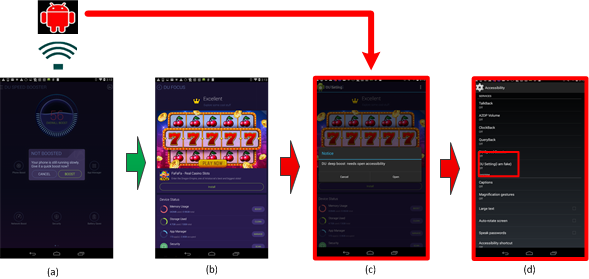
\includegraphics[width = 3.0in]{pic2.png}
\caption{\label{}Example of Dialog Escalation with PEC threats}
\end{figure}

\begin{figure}
\centering
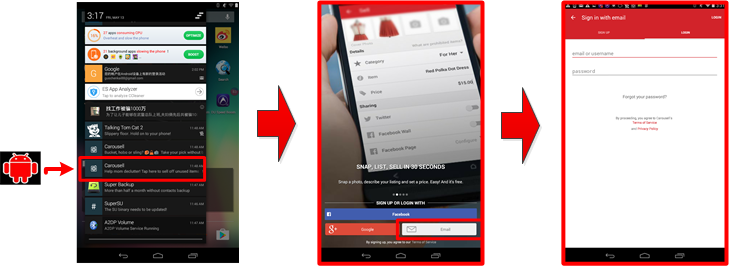
\includegraphics[width = 3.0in]{pic3.png}
\caption{\label{}Example of Notification Forgery with PEC threats}
\end{figure}

\begin{figure}
\centering
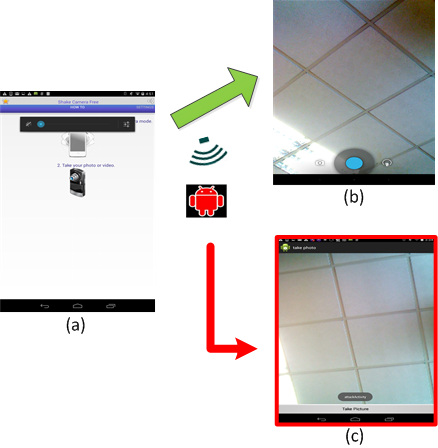
\includegraphics[width = 3.0in]{pic4.png}
\caption{\label{}Example of Shaking Spoofing with PEC threats}
\end{figure}

\begin{figure}
\centering
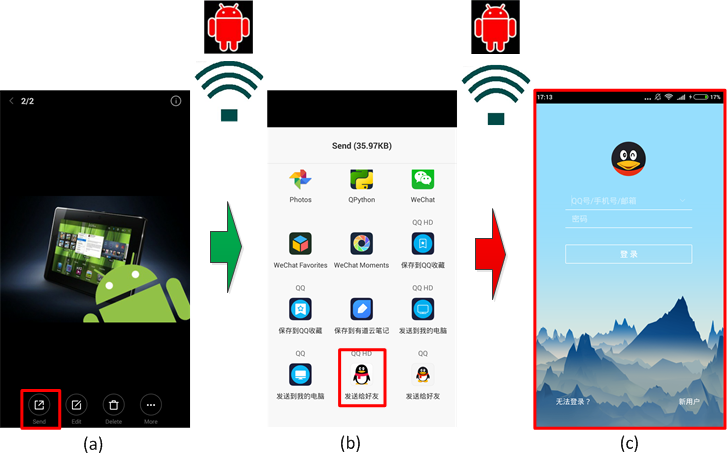
\includegraphics[width = 3.0in]{pic5.png}
\caption{\label{}Example of Activity Phishing with PEC threats}
\end{figure}


In this section, we present several representative exploits of the PEC weakness against the real-world apps. 
We demonstrate 1) how these exploits can be used to 
pinpoint a precise timing for GUI phishing attacks, and more importantly, 
2) how an attacker who has learnt the control flow information of the victim apps 
 can turn his easily-observable phishing attacks into unnoticeable ones. 
All the presented attacks have been tested on Android versions 3.*, 4.* and 5.*. 
\baigd{@Chenkai: check here}


%In this section, we present several representative attacks against the real-world apps
%In order to understand the attack feasibility of PEC threats, we explore typical types of attacks and present a detailed description of them in this section. Here, we represent one type of attack aiming to each display-sink as a fundamental exploration effort. We can foresee more attack types will continually emerge once the PEC threats are commonly noticed by attackers. 

%Following represents typical attacks forms that utilizes the PEC of victim app or PEC itself. According to the display-sink a PEC ends to, we representatively list several main types of attack examples, namely dialog \& toast privilege escalation, notification forgery, shaking-display spoofing and activity phishing. 

\subsubsection{Phishing Attacks Against Critical Dialog/Toast} \label{subsubsec:dialogattack}

%A typical implementation of above logic is represented as following:
%\begin{figure}
%\centering
%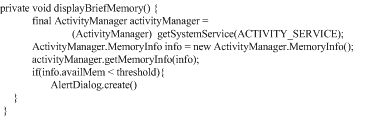
\includegraphics[width = 3.0in]{code1.png}
%\caption{\label{}control-flow}
%\end{figure}

In Android, Both of Dialog and Toast~(D\&T for short) 
act as a type of window display for notifying users the intermediate results or alert information when a particular event happens. 
Existing malicious apps~\cite{@chenkai: need citation here} spoof D\&Ts and pop up them occasionally or periodically, 
and once they are clicked, ... \baigd{@chenkai: add the consequence here.}
However, those D\&Ts are almost popped up at a wrong timing and they would inevitably arise the user's suspicion. 




%Previous attacks haven't pay enough attention to Dialog and Toast since the size of information carried by them is too small to make considerable security impact. Most of existing attacks upon D\&T rely on fooling user by a lure surface, which emerges in a sudden way that inevitably arises user's suspicion. In contrast, exploiting PEC threats is able to control the attack timing in reasonable scenes.


D\&Ts mostly are used for prompting the users about the real-time status of the app execution or system-level resources such as battery, memory and voice. 
Most of these statuses are triggered by the public events --- for example, Android system broadcast a \texttt{BATTERY\_LOW} event to 
indicate low battery condition on the device, and this event can be globally received. 
To make the problem even worse, 
because these events are usually related to the critical system-level status, 
the users tend to confirm the prompted actions~(by clicking ``Yes'' or ``OK''). 
In consequence, the success chance of the phishing attack with a spoofing D\&T increases. 

 %by apps). Therefore, a PEC threat contained by the D\&T or Toast holder  provides an indirect way for attacker understanding the popping up timing of certain D\&T and Toast. Further, attackers can employ user's trust of such D\&T holder to get the same trust for their adversaries.
%\textbf{PEC analysis.} %Once a public event is received, an adversary app would be easy to predict the time when a dialog or toast really emerges as long as the targeted app lacks of complex condition constrains in its control flow of the key callbacks. 
%Compared to sensitive information, D\&T are more likely to reflect real-time status about either app execution or system relevant resources such as \textit{battery}, \textit{memory}, \textit{voice}, etc. However, most of these statuses are closely connected to PE trigger (e.g., system will send BATTERY\_LOW event to indicate low battery condition on the device, which can be received by ordinary apps). Therefore, a PEC threat contained by the D\&T or Toast holder  provides an indirect way for attacker understanding the popping up timing of certain D\&T and Toast. Further, attackers can employ user's trust of such D\&T holder to get the same trust for their adversaries.

Based on these logic, we have studied the most popular
system management apps~(including \textsf{DU Speed Booster}, \textsf{Avast Cleanup}, etc.) which 
are typical apps that mainly process the system-level settings and frequently prompt the users for system running states. 
In this section, we take the process that \textsf{DU Speed Booster}~(denoted by \du hereafter) handles the storage status as an illustration example. 
\du is a system optimizer app which has accumulated more that 100 million installs. 


\paragraph{Working Model of Event-to-D\&T Control}
There exists a control flow from the PEC to the critical D\&Ts in \du, which working in the following way. 
\begin{itemize}
    \item Step \ding{172}. Once \du is started, it dynamically registers a broadcast receiver in the life-cycle event callback \texttt{onCreate} of its main Activity. 
    \item Step \ding{173}. This receiver aims to capture a public event named \texttt{DEVICE\_STORAGE\_LOW}. 
This event is broadcast by the system 
when the free storage on the device decreases to a level lower than a given level. 
    \item Step \ding{174}. 
Once this event is received by the receiver, the PEC \texttt{onReceiver} in this receiver pops up an alert dialog 
with short alarm messages like \emph{"Your phone is running slowly. Give it a deep boost now?"} and 
%, the D\&T can be predicted to be popped up on foreground in seconds. The PEC threats here assists to expose the certain knowledge about running stage (
\emph{"Hey! I have prepared to release the occupied storage!"}.  
%of such system management apps.
    \item Step \ding{175}. If the user confirms it, \du will transfer to process storage releasing. 
\end{itemize}


%and request user's decision whether to release the wasted occupation. If user  agree button, a new process launched by the manager app starts running.

%these kinds of notices are sent by pre-installed or system manager apps. Also, users are with fully trust for these apps in security part because they are professional and have numerous of users. However, this trust acts as a big opportunity that can be exploited to achieve the attack goal in attacker's eyes.

%The key point is the memory status(info.availMem) are public resources and can be obtained by any app installed in the device without any permission request. Moreover, the implementation control flow is designed so simple that 
%the condition logic and variable "threshold" could be easily reconstructed in an adversary app. A experienced attacker could also obtain the these key logic and variables through reverse-engineering and binary analysis. As a result, the condition "info.availMem < threshold" as a public events makes the function "AlertDialog.create()" a PEC, and attackers are able to judge the creating time of the AlerDialog from its own reconstructed adversary app installed in the same device.

\paragraph{The Attack}
The goal of the attacker is to pop up a spoofing dialog which if is confirmed, 
the user will be directed to a system setting page desired by the attacker. 
The spoofing dialog can deceive the user into thinking the storage releasing action requires the 
user to manually do some settings. 
Since the user believes that he is directed to this page by \du, he is highly likely to 
confirm the setting desired by the attackers. 
A good example of the setting pages is the \texttt{Accessibility Service} setting~(shown in Figure~\ref{@snapshot here}). 
The \texttt{Accessibility Service} serves as a specific functionality supplied by Android to help disabled people conveniently 
obtain the component status and handle the device operations. 
Android supports even richer interfaces of the \texttt{Accessibility Service} after version 4.0, which on the other side arises higher security risk. 
Hence, it is restricted by Android that all relevant implementations have to be engaged under the user's manual grant through the setting page.
If granted this permission, the malicious app becomes able to \baigd{@chenkai: emphasize why this permission is dangerous}. 

A critical factor to achieve this attack is the timing. 
For example, an intuitive way is to pop up the spoofing dialog once \du is detected to be running on foreground. 
The problem is that it may raises the user's suspicion if \du does not actually conduct storage releasing after foreground interface switches back 
from the system setting page. 
In contrast, this problem can be prevented if the spoofing dialog is popped up after step \ding{174}. 
The malicious app can pinpoint this timing via the following steps. 

\begin{itemize}
    \item Step \ding{182}. The malicious app starts a background service which monitors whether \du is in running on foreground, namely whether the PEC \texttt{onCreate} happens. 
    \item Step \ding{183}. If \ding{182} happens, the malicious app then registers a receiver to monitor whether \texttt{DEVICE\_STORAGE\_LOW} occurs.  
    \item Step \ding{184}. If \ding{183} happens, the malicious app pops up a spoofing a dialog immediately after the \du's dialog has been popped up --- this is possible to achieve given that the attacker can measure the length of time period \du takes to pop up its dialog after \ding{183} happens. 
    At this point, the spoofing dialog covers \du's dialog.
    It can pretend as the latter and say that \emph{``\du needs \texttt{Accessibility Service} permission for storage releasing.''} . 
    \item Step \ding{185}.  Once user clicks \textit{Agree} button, a \textit{Accessibility Service} setting page is automatically opened on the foreground using \texttt{Setting.ACTION\_ACCESSIBILITY\_SETTINGS}. 
\end{itemize}

\subsubsection{Notification Forgery}
The Notification in Android normally works for showing the received updated message and the task progress information, which is somehow similar as D\&T. Different from the latter, the user is not necessary to immediately handle the message sent by a Notification. Instead, the developer uses \texttt{PendingIntent} to handle intent in the future, which is upon when user clicks the Notification. 

 %in the Notification Drawer

%Again, a Notification would not disappear in seconds as the Toast does until user handles it. The user could handle it at any time they like, which gives attackers enough time to forge a fake one escaping user's attention. Here we introduce two common used situations. 

\textbf{PEC analysis.}
Most of the market apps currently are based on CS (Client-Server) pattern, and the server needs to frequently push the updating data to the client (app installed in user's device). The client keeps running a service in the background to communicate with the server. Normally, this push-receive mechanism is implemented by specialized module with high-level security protection that makes it hard to get any push status by other apps. However, since the status of client service is publicly opened, adversary also could exploit it to fool the user in an indirect way. 

First, through pre-analysing the service of victim app for handling the pushed data, an attacker can judge whether it's PECs links to a Notification display or not. If the life-cycle PEC onCreate() indeed links to a Notification sending logic, the adversary can receive a signal from the victim service that it keeps receiving the pushed data and sending Notification. Given that knowledge, the adversary judges that a same Notification sending action is hard to arise user's suspicion.   

%Besides that, another PEC threat emerges when the user clicks on the Notification. There are two PEs within this process. One is the change of the Notification Drawer serves as the PE, causing other apps can deceive it through the open APIs provided by \texttt{NotificationManager} without permission request.

\textbf{Attack Implementation.}
Consider the app Carousell, a popular goods-trading platform that frequently sends Notification notifying it's new selling information to user. Normally, Carousell builds a resident service \texttt{PendingIntentCallbackService} running on the background. When an adversary observes it's running, a fake Notification constructed with the same resources and framework as original Carousell did(Figure * (a)). Fortunately, Android system currently allows a developer to arbitrarily build the appearance of its own Notification, especially the icon and content. The relevant open APIs are provided in the \texttt{Builder} class (e.g., \texttt{setContentTitle()}, \texttt{setContentText()}, \texttt{setSmallIcon()}, etc.). Different with the benign Notification, the fake one is connected to a carefully constructed \textit{Carousell login} page that needs user input their Carousell account(even the account of third-party single sign-on Facebook and Google)(Figure * (b)\&(c)). When the user opens the Notification Drawer, there are several very similar Notifications listing there(as Figure * (a) shows). If the user chooses the fake one and tries to log in the Carousell account, the user name and password will be delivered to the attacker through network.


%\# Notice. Another important usage of the Notification is to notify users update status from a specific app or the device system. For instance, the QPtyhon(An app for python debugging on Android) would perform a log Notification when the onDestroy() lifecycle function in the MainActivity happens. However, since the onDestroy() is invoked when the MainActivity is destroyed, a third-party app uses the getRunningAppProcesses()(offered by ActivityManager) function to judge it. Thus, the onDestroy() belongs to the PEC as well. Attackers could capture the time of such Notification emergence and even the time user triggers the Notification(when the targeted Notification is dismissed and corresponding app starts running.)by analysis from getActiveNotifications() offered by NotificationManager(after Android 4.3) 

%Once it happens, the adversary would predict the notice Dialog will pop up in a few seconds(Figure *(a)).

% After that, it shows a Dialog tip(Figure *(c)) to tell user the corresponding Accessibility Service have to be grant to complete the data clean task, and then opens the Accessibility Service setting page using "Setting.ACTION\_ACCESSIBILITY\_SETTINGS" intent like Figure *(d) did. In the setting page, an attack service with a confused name "DU deep boost" fool user about this attack. At last, the adversary app gets the grant and could engage further attacks. 



%In order to clearly illustrate the attack process, first the threat model need to be depicted.
%Suppose that we have a victim app installed in a given device, and it contains corresponding callback threats vulnerabilities. Besides, suppose that we have an adversary app installed in the same device and start its service running on the background stealthily. The goal of our adversary app is to engage diverse attacks through the victim app. In theory, the adversary app need not apply any permission when it is installed. However, in practice, it needs to apply some  common-used permissions like "Internet" and insensitive permissions like "batter related permission" according to the attack type. The adversary needs to visually conceal its behaviours from users and also minimize its impact on the device performance. 

%The adversary is supposed having the capability of using public available resources and analysing them on the fly. Again, it should stay aware of the running states of apps and some particular services. As introduced in "Callback State Model", this capability can be obtained by particular methods within ActivityManager class.

%\section{Attacking PEC Weakness}

%\subsection{Exploiting Condition}
%\paragraph{App Description}
%\paragraph{Timer}

In this section, we present several concrete attacks against real-world apps which have the PEC weakness. 
These attacks demonstrate that exploiting PEC weakness helps the attacker pinpoint the timing to conduct attacks. 


\subsection{Threat Model} \label{subsec:threat}

In our threat model, the attacker is able to conduct an offline control analysis before conducting the attack on the devices. 
This offline analysis allows the attacker to learn the PEC models of the publicly available apps~(e.g., the apps published in Google Play market). 
The attacker is able to install his attack payloads into the victim devices, through either luring the users into installing his apps or injecting his code into 
the installed benign apps. 
%Our analysis is built on arbitrary Android device environment with an adversary app stealthily running on the background out of user's awareness.  
%The adversary needs to conceal its behaviours and minimize its impact on the device performance. 
The attack payloads can be stealthily run on the background out of the user's awareness. 
The attacker also has to conceal its behaviours and minimize its impact on the device performance. 
% \baigd{comments: how? the attacker needs to read /proc file periodically. You may have to measure the performance/battery overhead}
The goal of attackers is to conduct the \emph{event hijacking} exploiting certain victim app 
and to achieve its malicious purpose~(e.g., to obtain user's sensitive data and to escalate access privilege). 
Similar to related work~\cite{chen2014peeking,ren2015towards}, 
the adversary app is supposed to be installed 
%without requesting any permissions except 
with only a couple of commonly-used permissions like \texttt{INTERNENT}. 
%which is commonly required by existing attacks on Android OS
%\cite{chen2014peeking}\cite{ren2015towards}. 
In some special scenarios, insensitive permissions for users such as \texttt{BATTERY\_STATS} are also allowed to be requested in order to 
%predict \baigd{What do you mean here?} victim's related \emph{control confidentiality}. 
observe the occurrence of the public events.  


%The adversary is supposed having the capability of using public  and analysing them on the fly. Again, . As introduced in "Callback State Model", this capability can be obtained by particular methods within ActivityManager class.
%it should stay aware of the running states of apps and some particular services

\subsection{Attacks Exploiting the PEC Threats}

\begin{figure}
\centering
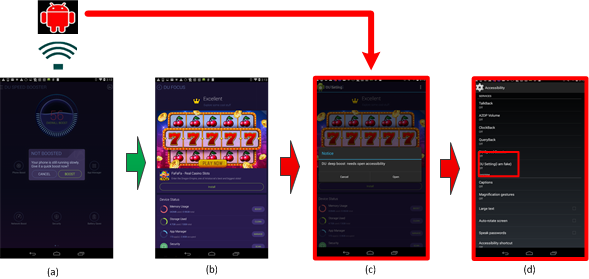
\includegraphics[width = 3.0in]{pic2.png}
\caption{\label{}Example of Dialog Escalation with PEC threats}
\end{figure}

\begin{figure}
\centering
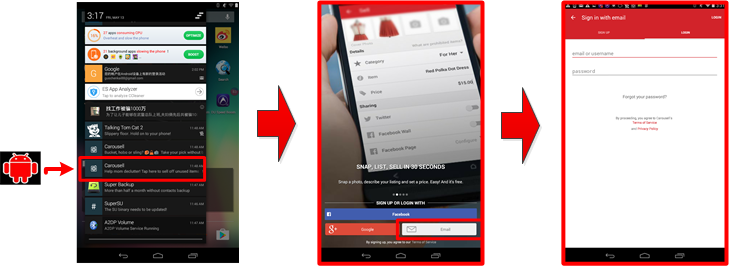
\includegraphics[width = 3.0in]{pic3.png}
\caption{\label{}Example of Notification Forgery with PEC threats}
\end{figure}

\begin{figure}
\centering
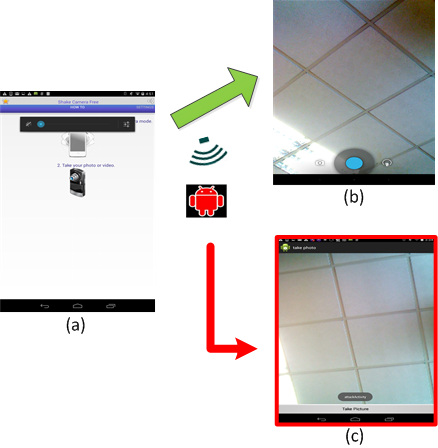
\includegraphics[width = 3.0in]{pic4.png}
\caption{\label{}Example of Shaking Spoofing with PEC threats}
\end{figure}

\begin{figure}
\centering
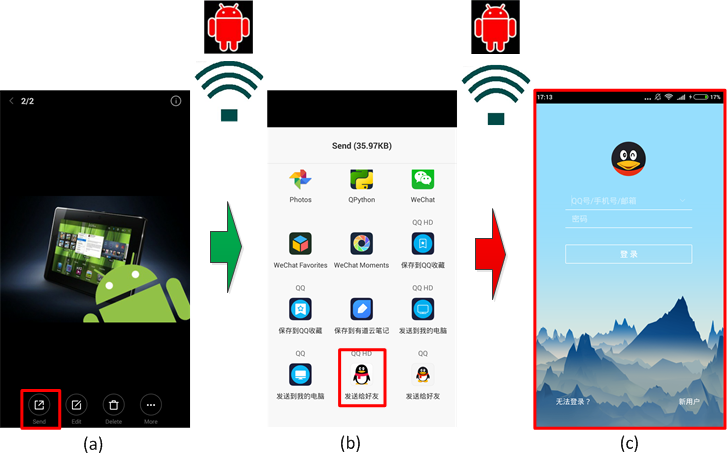
\includegraphics[width = 3.0in]{pic5.png}
\caption{\label{}Example of Activity Phishing with PEC threats}
\end{figure}


In this section, we present several representative exploits of the PEC weakness against the real-world apps. 
We demonstrate 1) how these exploits can be used to 
pinpoint a precise timing for GUI phishing attacks, and more importantly, 
2) how an attacker who has learnt the control flow information of the victim apps 
 can turn his easily-observable phishing attacks into unnoticeable ones. 
All the presented attacks have been tested on Android versions 3.*, 4.* and 5.*. 
\baigd{@Chenkai: check here}


%In this section, we present several representative attacks against the real-world apps
%In order to understand the attack feasibility of PEC threats, we explore typical types of attacks and present a detailed description of them in this section. Here, we represent one type of attack aiming to each display-sink as a fundamental exploration effort. We can foresee more attack types will continually emerge once the PEC threats are commonly noticed by attackers. 

%Following represents typical attacks forms that utilizes the PEC of victim app or PEC itself. According to the display-sink a PEC ends to, we representatively list several main types of attack examples, namely dialog \& toast privilege escalation, notification forgery, shaking-display spoofing and activity phishing. 

\subsubsection{Phishing Attacks Against Critical Dialog/Toast} \label{subsubsec:dialogattack}

%A typical implementation of above logic is represented as following:
%\begin{figure}
%\centering
%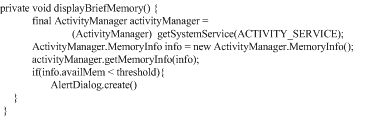
\includegraphics[width = 3.0in]{code1.png}
%\caption{\label{}control-flow}
%\end{figure}

In Android, Both of Dialog and Toast~(D\&T for short) 
act as a type of window display for notifying users the intermediate results or alert information when a particular event happens. 
Existing malicious apps~\cite{@chenkai: need citation here} spoof D\&Ts and pop up them occasionally or periodically, 
and once they are clicked, ... \baigd{@chenkai: add the consequence here.}
However, those D\&Ts are almost popped up at a wrong timing and they would inevitably arise the user's suspicion. 




%Previous attacks haven't pay enough attention to Dialog and Toast since the size of information carried by them is too small to make considerable security impact. Most of existing attacks upon D\&T rely on fooling user by a lure surface, which emerges in a sudden way that inevitably arises user's suspicion. In contrast, exploiting PEC threats is able to control the attack timing in reasonable scenes.


D\&Ts mostly are used for prompting the users about the real-time status of the app execution or system-level resources such as battery, memory and voice. 
Most of these statuses are triggered by the public events --- for example, Android system broadcast a \texttt{BATTERY\_LOW} event to 
indicate low battery condition on the device, and this event can be globally received. 
To make the problem even worse, 
because these events are usually related to the critical system-level status, 
the users tend to confirm the prompted actions~(by clicking ``Yes'' or ``OK''). 
In consequence, the success chance of the phishing attack with a spoofing D\&T increases. 

 %by apps). Therefore, a PEC threat contained by the D\&T or Toast holder  provides an indirect way for attacker understanding the popping up timing of certain D\&T and Toast. Further, attackers can employ user's trust of such D\&T holder to get the same trust for their adversaries.
%\textbf{PEC analysis.} %Once a public event is received, an adversary app would be easy to predict the time when a dialog or toast really emerges as long as the targeted app lacks of complex condition constrains in its control flow of the key callbacks. 
%Compared to sensitive information, D\&T are more likely to reflect real-time status about either app execution or system relevant resources such as \textit{battery}, \textit{memory}, \textit{voice}, etc. However, most of these statuses are closely connected to PE trigger (e.g., system will send BATTERY\_LOW event to indicate low battery condition on the device, which can be received by ordinary apps). Therefore, a PEC threat contained by the D\&T or Toast holder  provides an indirect way for attacker understanding the popping up timing of certain D\&T and Toast. Further, attackers can employ user's trust of such D\&T holder to get the same trust for their adversaries.

Based on these logic, we have studied the most popular
system management apps~(including \textsf{DU Speed Booster}, \textsf{Avast Cleanup}, etc.) which 
are typical apps that mainly process the system-level settings and frequently prompt the users for system running states. 
In this section, we take the process that \textsf{DU Speed Booster}~(denoted by \du hereafter) handles the storage status as an illustration example. 
\du is a system optimizer app which has accumulated more that 100 million installs. 


\paragraph{Working Model of Event-to-D\&T Control}
There exists a control flow from the PEC to the critical D\&Ts in \du, which working in the following way. 
\begin{itemize}
    \item Step \ding{172}. Once \du is started, it dynamically registers a broadcast receiver in the life-cycle event callback \texttt{onCreate} of its main Activity. 
    \item Step \ding{173}. This receiver aims to capture a public event named \texttt{DEVICE\_STORAGE\_LOW}. 
This event is broadcast by the system 
when the free storage on the device decreases to a level lower than a given level. 
    \item Step \ding{174}. 
Once this event is received by the receiver, the PEC \texttt{onReceiver} in this receiver pops up an alert dialog 
with short alarm messages like \emph{"Your phone is running slowly. Give it a deep boost now?"} and 
%, the D\&T can be predicted to be popped up on foreground in seconds. The PEC threats here assists to expose the certain knowledge about running stage (
\emph{"Hey! I have prepared to release the occupied storage!"}.  
%of such system management apps.
    \item Step \ding{175}. If the user confirms it, \du will transfer to process storage releasing. 
\end{itemize}


%and request user's decision whether to release the wasted occupation. If user  agree button, a new process launched by the manager app starts running.

%these kinds of notices are sent by pre-installed or system manager apps. Also, users are with fully trust for these apps in security part because they are professional and have numerous of users. However, this trust acts as a big opportunity that can be exploited to achieve the attack goal in attacker's eyes.

%The key point is the memory status(info.availMem) are public resources and can be obtained by any app installed in the device without any permission request. Moreover, the implementation control flow is designed so simple that 
%the condition logic and variable "threshold" could be easily reconstructed in an adversary app. A experienced attacker could also obtain the these key logic and variables through reverse-engineering and binary analysis. As a result, the condition "info.availMem < threshold" as a public events makes the function "AlertDialog.create()" a PEC, and attackers are able to judge the creating time of the AlerDialog from its own reconstructed adversary app installed in the same device.

\paragraph{The Attack}
The goal of the attacker is to pop up a spoofing dialog which if is confirmed, 
the user will be directed to a system setting page desired by the attacker. 
The spoofing dialog can deceive the user into thinking the storage releasing action requires the 
user to manually do some settings. 
Since the user believes that he is directed to this page by \du, he is highly likely to 
confirm the setting desired by the attackers. 
A good example of the setting pages is the \texttt{Accessibility Service} setting~(shown in Figure~\ref{@snapshot here}). 
The \texttt{Accessibility Service} serves as a specific functionality supplied by Android to help disabled people conveniently 
obtain the component status and handle the device operations. 
Android supports even richer interfaces of the \texttt{Accessibility Service} after version 4.0, which on the other side arises higher security risk. 
Hence, it is restricted by Android that all relevant implementations have to be engaged under the user's manual grant through the setting page.
If granted this permission, the malicious app becomes able to \baigd{@chenkai: emphasize why this permission is dangerous}. 

A critical factor to achieve this attack is the timing. 
For example, an intuitive way is to pop up the spoofing dialog once \du is detected to be running on foreground. 
The problem is that it may raises the user's suspicion if \du does not actually conduct storage releasing after foreground interface switches back 
from the system setting page. 
In contrast, this problem can be prevented if the spoofing dialog is popped up after step \ding{174}. 
The malicious app can pinpoint this timing via the following steps. 

\begin{itemize}
    \item Step \ding{182}. The malicious app starts a background service which monitors whether \du is in running on foreground, namely whether the PEC \texttt{onCreate} happens. 
    \item Step \ding{183}. If \ding{182} happens, the malicious app then registers a receiver to monitor whether \texttt{DEVICE\_STORAGE\_LOW} occurs.  
    \item Step \ding{184}. If \ding{183} happens, the malicious app pops up a spoofing a dialog immediately after the \du's dialog has been popped up --- this is possible to achieve given that the attacker can measure the length of time period \du takes to pop up its dialog after \ding{183} happens. 
    At this point, the spoofing dialog covers \du's dialog.
    It can pretend as the latter and say that \emph{``\du needs \texttt{Accessibility Service} permission for storage releasing.''} . 
    \item Step \ding{185}.  Once user clicks \textit{Agree} button, a \textit{Accessibility Service} setting page is automatically opened on the foreground using \texttt{Setting.ACTION\_ACCESSIBILITY\_SETTINGS}. 
\end{itemize}

\subsubsection{Notification Forgery}
The Notification in Android normally works for showing the received updated message and the task progress information, which is somehow similar as D\&T. Different from the latter, the user is not necessary to immediately handle the message sent by a Notification. Instead, the developer uses \texttt{PendingIntent} to handle intent in the future, which is upon when user clicks the Notification. 

 %in the Notification Drawer

%Again, a Notification would not disappear in seconds as the Toast does until user handles it. The user could handle it at any time they like, which gives attackers enough time to forge a fake one escaping user's attention. Here we introduce two common used situations. 

\textbf{PEC analysis.}
Most of the market apps currently are based on CS (Client-Server) pattern, and the server needs to frequently push the updating data to the client (app installed in user's device). The client keeps running a service in the background to communicate with the server. Normally, this push-receive mechanism is implemented by specialized module with high-level security protection that makes it hard to get any push status by other apps. However, since the status of client service is publicly opened, adversary also could exploit it to fool the user in an indirect way. 

First, through pre-analysing the service of victim app for handling the pushed data, an attacker can judge whether it's PECs links to a Notification display or not. If the life-cycle PEC onCreate() indeed links to a Notification sending logic, the adversary can receive a signal from the victim service that it keeps receiving the pushed data and sending Notification. Given that knowledge, the adversary judges that a same Notification sending action is hard to arise user's suspicion.   

%Besides that, another PEC threat emerges when the user clicks on the Notification. There are two PEs within this process. One is the change of the Notification Drawer serves as the PE, causing other apps can deceive it through the open APIs provided by \texttt{NotificationManager} without permission request.

\textbf{Attack Implementation.}
Consider the app Carousell, a popular goods-trading platform that frequently sends Notification notifying it's new selling information to user. Normally, Carousell builds a resident service \texttt{PendingIntentCallbackService} running on the background. When an adversary observes it's running, a fake Notification constructed with the same resources and framework as original Carousell did(Figure * (a)). Fortunately, Android system currently allows a developer to arbitrarily build the appearance of its own Notification, especially the icon and content. The relevant open APIs are provided in the \texttt{Builder} class (e.g., \texttt{setContentTitle()}, \texttt{setContentText()}, \texttt{setSmallIcon()}, etc.). Different with the benign Notification, the fake one is connected to a carefully constructed \textit{Carousell login} page that needs user input their Carousell account(even the account of third-party single sign-on Facebook and Google)(Figure * (b)\&(c)). When the user opens the Notification Drawer, there are several very similar Notifications listing there(as Figure * (a) shows). If the user chooses the fake one and tries to log in the Carousell account, the user name and password will be delivered to the attacker through network.


%\# Notice. Another important usage of the Notification is to notify users update status from a specific app or the device system. For instance, the QPtyhon(An app for python debugging on Android) would perform a log Notification when the onDestroy() lifecycle function in the MainActivity happens. However, since the onDestroy() is invoked when the MainActivity is destroyed, a third-party app uses the getRunningAppProcesses()(offered by ActivityManager) function to judge it. Thus, the onDestroy() belongs to the PEC as well. Attackers could capture the time of such Notification emergence and even the time user triggers the Notification(when the targeted Notification is dismissed and corresponding app starts running.)by analysis from getActiveNotifications() offered by NotificationManager(after Android 4.3) 

%Once it happens, the adversary would predict the notice Dialog will pop up in a few seconds(Figure *(a)).

% After that, it shows a Dialog tip(Figure *(c)) to tell user the corresponding Accessibility Service have to be grant to complete the data clean task, and then opens the Accessibility Service setting page using "Setting.ACTION\_ACCESSIBILITY\_SETTINGS" intent like Figure *(d) did. In the setting page, an attack service with a confused name "DU deep boost" fool user about this attack. At last, the adversary app gets the grant and could engage further attacks. 



%In order to clearly illustrate the attack process, first the threat model need to be depicted.
%Suppose that we have a victim app installed in a given device, and it contains corresponding callback threats vulnerabilities. Besides, suppose that we have an adversary app installed in the same device and start its service running on the background stealthily. The goal of our adversary app is to engage diverse attacks through the victim app. In theory, the adversary app need not apply any permission when it is installed. However, in practice, it needs to apply some  common-used permissions like "Internet" and insensitive permissions like "batter related permission" according to the attack type. The adversary needs to visually conceal its behaviours from users and also minimize its impact on the device performance. 

%The adversary is supposed having the capability of using public available resources and analysing them on the fly. Again, it should stay aware of the running states of apps and some particular services. As introduced in "Callback State Model", this capability can be obtained by particular methods within ActivityManager class.

%\section{Attacking PEC Weakness}

%\subsection{Exploiting Condition}
%\paragraph{App Description}
%\paragraph{Timer}

In this section, we present several concrete attacks against real-world apps which have the PEC weakness. 
These attacks demonstrate that exploiting PEC weakness helps the attacker pinpoint the timing to conduct attacks. 


\subsection{Threat Model} \label{subsec:threat}

In our threat model, the attacker is able to conduct an offline control analysis before conducting the attack on the devices. 
This offline analysis allows the attacker to learn the PEC models of the publicly available apps~(e.g., the apps published in Google Play market). 
The attacker is able to install his attack payloads into the victim devices, through either luring the users into installing his apps or injecting his code into 
the installed benign apps. 
%Our analysis is built on arbitrary Android device environment with an adversary app stealthily running on the background out of user's awareness.  
%The adversary needs to conceal its behaviours and minimize its impact on the device performance. 
The attack payloads can be stealthily run on the background out of the user's awareness. 
The attacker also has to conceal its behaviours and minimize its impact on the device performance. 
% \baigd{comments: how? the attacker needs to read /proc file periodically. You may have to measure the performance/battery overhead}
The goal of attackers is to conduct the \emph{event hijacking} exploiting certain victim app 
and to achieve its malicious purpose~(e.g., to obtain user's sensitive data and to escalate access privilege). 
Similar to related work~\cite{chen2014peeking,ren2015towards}, 
the adversary app is supposed to be installed 
%without requesting any permissions except 
with only a couple of commonly-used permissions like \texttt{INTERNENT}. 
%which is commonly required by existing attacks on Android OS
%\cite{chen2014peeking}\cite{ren2015towards}. 
In some special scenarios, insensitive permissions for users such as \texttt{BATTERY\_STATS} are also allowed to be requested in order to 
%predict \baigd{What do you mean here?} victim's related \emph{control confidentiality}. 
observe the occurrence of the public events.  


%The adversary is supposed having the capability of using public  and analysing them on the fly. Again, . As introduced in "Callback State Model", this capability can be obtained by particular methods within ActivityManager class.
%it should stay aware of the running states of apps and some particular services

\subsection{Attacks Exploiting the PEC Threats}

\begin{figure}
\centering
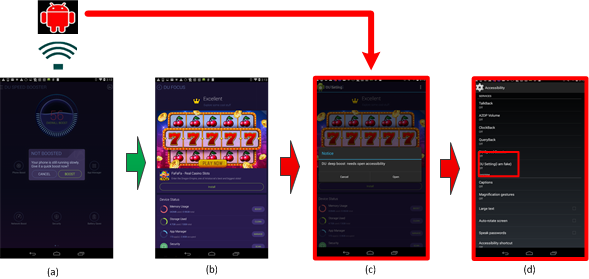
\includegraphics[width = 3.0in]{pic2.png}
\caption{\label{}Example of Dialog Escalation with PEC threats}
\end{figure}

\begin{figure}
\centering
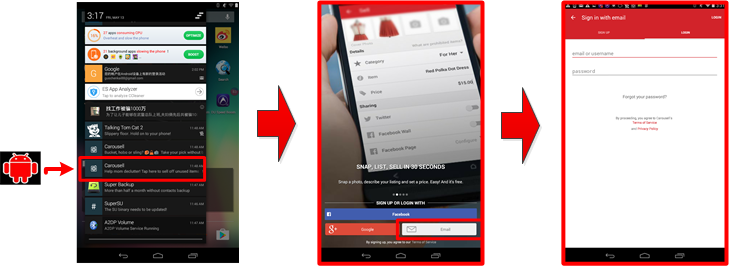
\includegraphics[width = 3.0in]{pic3.png}
\caption{\label{}Example of Notification Forgery with PEC threats}
\end{figure}

\begin{figure}
\centering
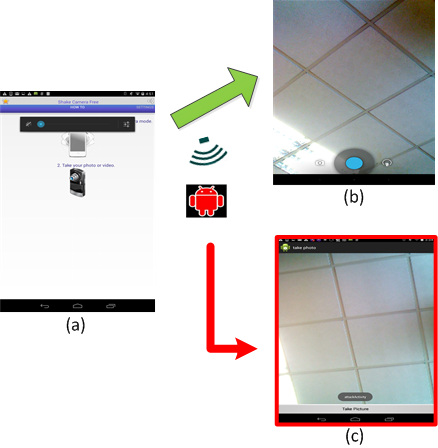
\includegraphics[width = 3.0in]{pic4.png}
\caption{\label{}Example of Shaking Spoofing with PEC threats}
\end{figure}

\begin{figure}
\centering
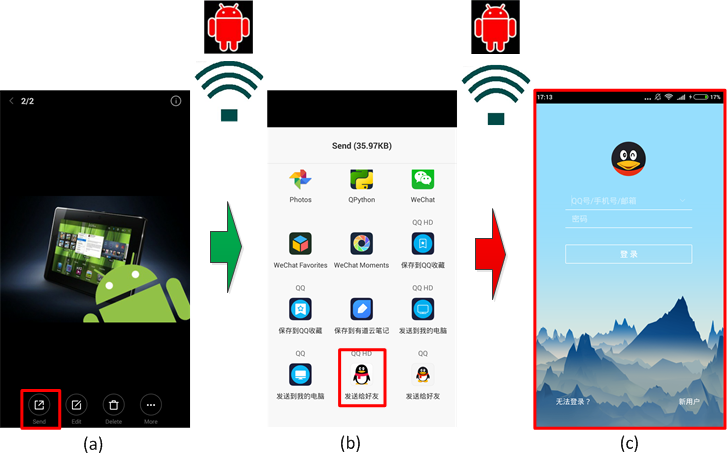
\includegraphics[width = 3.0in]{pic5.png}
\caption{\label{}Example of Activity Phishing with PEC threats}
\end{figure}


In this section, we present several representative exploits of the PEC weakness against the real-world apps. 
We demonstrate 1) how these exploits can be used to 
pinpoint a precise timing for GUI phishing attacks, and more importantly, 
2) how an attacker who has learnt the control flow information of the victim apps 
 can turn his easily-observable phishing attacks into unnoticeable ones. 
All the presented attacks have been tested on Android versions 3.*, 4.* and 5.*. 
\baigd{@Chenkai: check here}


%In this section, we present several representative attacks against the real-world apps
%In order to understand the attack feasibility of PEC threats, we explore typical types of attacks and present a detailed description of them in this section. Here, we represent one type of attack aiming to each display-sink as a fundamental exploration effort. We can foresee more attack types will continually emerge once the PEC threats are commonly noticed by attackers. 

%Following represents typical attacks forms that utilizes the PEC of victim app or PEC itself. According to the display-sink a PEC ends to, we representatively list several main types of attack examples, namely dialog \& toast privilege escalation, notification forgery, shaking-display spoofing and activity phishing. 

\subsubsection{Phishing Attacks Against Critical Dialog/Toast} \label{subsubsec:dialogattack}

%A typical implementation of above logic is represented as following:
%\begin{figure}
%\centering
%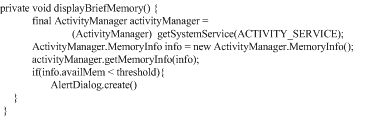
\includegraphics[width = 3.0in]{code1.png}
%\caption{\label{}control-flow}
%\end{figure}

In Android, Both of Dialog and Toast~(D\&T for short) 
act as a type of window display for notifying users the intermediate results or alert information when a particular event happens. 
Existing malicious apps~\cite{@chenkai: need citation here} spoof D\&Ts and pop up them occasionally or periodically, 
and once they are clicked, ... \baigd{@chenkai: add the consequence here.}
However, those D\&Ts are almost popped up at a wrong timing and they would inevitably arise the user's suspicion. 




%Previous attacks haven't pay enough attention to Dialog and Toast since the size of information carried by them is too small to make considerable security impact. Most of existing attacks upon D\&T rely on fooling user by a lure surface, which emerges in a sudden way that inevitably arises user's suspicion. In contrast, exploiting PEC threats is able to control the attack timing in reasonable scenes.


D\&Ts mostly are used for prompting the users about the real-time status of the app execution or system-level resources such as battery, memory and voice. 
Most of these statuses are triggered by the public events --- for example, Android system broadcast a \texttt{BATTERY\_LOW} event to 
indicate low battery condition on the device, and this event can be globally received. 
To make the problem even worse, 
because these events are usually related to the critical system-level status, 
the users tend to confirm the prompted actions~(by clicking ``Yes'' or ``OK''). 
In consequence, the success chance of the phishing attack with a spoofing D\&T increases. 

 %by apps). Therefore, a PEC threat contained by the D\&T or Toast holder  provides an indirect way for attacker understanding the popping up timing of certain D\&T and Toast. Further, attackers can employ user's trust of such D\&T holder to get the same trust for their adversaries.
%\textbf{PEC analysis.} %Once a public event is received, an adversary app would be easy to predict the time when a dialog or toast really emerges as long as the targeted app lacks of complex condition constrains in its control flow of the key callbacks. 
%Compared to sensitive information, D\&T are more likely to reflect real-time status about either app execution or system relevant resources such as \textit{battery}, \textit{memory}, \textit{voice}, etc. However, most of these statuses are closely connected to PE trigger (e.g., system will send BATTERY\_LOW event to indicate low battery condition on the device, which can be received by ordinary apps). Therefore, a PEC threat contained by the D\&T or Toast holder  provides an indirect way for attacker understanding the popping up timing of certain D\&T and Toast. Further, attackers can employ user's trust of such D\&T holder to get the same trust for their adversaries.

Based on these logic, we have studied the most popular
system management apps~(including \textsf{DU Speed Booster}, \textsf{Avast Cleanup}, etc.) which 
are typical apps that mainly process the system-level settings and frequently prompt the users for system running states. 
In this section, we take the process that \textsf{DU Speed Booster}~(denoted by \du hereafter) handles the storage status as an illustration example. 
\du is a system optimizer app which has accumulated more that 100 million installs. 


\paragraph{Working Model of Event-to-D\&T Control}
There exists a control flow from the PEC to the critical D\&Ts in \du, which working in the following way. 
\begin{itemize}
    \item Step \ding{172}. Once \du is started, it dynamically registers a broadcast receiver in the life-cycle event callback \texttt{onCreate} of its main Activity. 
    \item Step \ding{173}. This receiver aims to capture a public event named \texttt{DEVICE\_STORAGE\_LOW}. 
This event is broadcast by the system 
when the free storage on the device decreases to a level lower than a given level. 
    \item Step \ding{174}. 
Once this event is received by the receiver, the PEC \texttt{onReceiver} in this receiver pops up an alert dialog 
with short alarm messages like \emph{"Your phone is running slowly. Give it a deep boost now?"} and 
%, the D\&T can be predicted to be popped up on foreground in seconds. The PEC threats here assists to expose the certain knowledge about running stage (
\emph{"Hey! I have prepared to release the occupied storage!"}.  
%of such system management apps.
    \item Step \ding{175}. If the user confirms it, \du will transfer to process storage releasing. 
\end{itemize}


%and request user's decision whether to release the wasted occupation. If user  agree button, a new process launched by the manager app starts running.

%these kinds of notices are sent by pre-installed or system manager apps. Also, users are with fully trust for these apps in security part because they are professional and have numerous of users. However, this trust acts as a big opportunity that can be exploited to achieve the attack goal in attacker's eyes.

%The key point is the memory status(info.availMem) are public resources and can be obtained by any app installed in the device without any permission request. Moreover, the implementation control flow is designed so simple that 
%the condition logic and variable "threshold" could be easily reconstructed in an adversary app. A experienced attacker could also obtain the these key logic and variables through reverse-engineering and binary analysis. As a result, the condition "info.availMem < threshold" as a public events makes the function "AlertDialog.create()" a PEC, and attackers are able to judge the creating time of the AlerDialog from its own reconstructed adversary app installed in the same device.

\paragraph{The Attack}
The goal of the attacker is to pop up a spoofing dialog which if is confirmed, 
the user will be directed to a system setting page desired by the attacker. 
The spoofing dialog can deceive the user into thinking the storage releasing action requires the 
user to manually do some settings. 
Since the user believes that he is directed to this page by \du, he is highly likely to 
confirm the setting desired by the attackers. 
A good example of the setting pages is the \texttt{Accessibility Service} setting~(shown in Figure~\ref{@snapshot here}). 
The \texttt{Accessibility Service} serves as a specific functionality supplied by Android to help disabled people conveniently 
obtain the component status and handle the device operations. 
Android supports even richer interfaces of the \texttt{Accessibility Service} after version 4.0, which on the other side arises higher security risk. 
Hence, it is restricted by Android that all relevant implementations have to be engaged under the user's manual grant through the setting page.
If granted this permission, the malicious app becomes able to \baigd{@chenkai: emphasize why this permission is dangerous}. 

A critical factor to achieve this attack is the timing. 
For example, an intuitive way is to pop up the spoofing dialog once \du is detected to be running on foreground. 
The problem is that it may raises the user's suspicion if \du does not actually conduct storage releasing after foreground interface switches back 
from the system setting page. 
In contrast, this problem can be prevented if the spoofing dialog is popped up after step \ding{174}. 
The malicious app can pinpoint this timing via the following steps. 

\begin{itemize}
    \item Step \ding{182}. The malicious app starts a background service which monitors whether \du is in running on foreground, namely whether the PEC \texttt{onCreate} happens. 
    \item Step \ding{183}. If \ding{182} happens, the malicious app then registers a receiver to monitor whether \texttt{DEVICE\_STORAGE\_LOW} occurs.  
    \item Step \ding{184}. If \ding{183} happens, the malicious app pops up a spoofing a dialog immediately after the \du's dialog has been popped up --- this is possible to achieve given that the attacker can measure the length of time period \du takes to pop up its dialog after \ding{183} happens. 
    At this point, the spoofing dialog covers \du's dialog.
    It can pretend as the latter and say that \emph{``\du needs \texttt{Accessibility Service} permission for storage releasing.''} . 
    \item Step \ding{185}.  Once user clicks \textit{Agree} button, a \textit{Accessibility Service} setting page is automatically opened on the foreground using \texttt{Setting.ACTION\_ACCESSIBILITY\_SETTINGS}. 
\end{itemize}

\subsubsection{Notification Forgery}
The Notification in Android normally works for showing the received updated message and the task progress information, which is somehow similar as D\&T. Different from the latter, the user is not necessary to immediately handle the message sent by a Notification. Instead, the developer uses \texttt{PendingIntent} to handle intent in the future, which is upon when user clicks the Notification. 

 %in the Notification Drawer

%Again, a Notification would not disappear in seconds as the Toast does until user handles it. The user could handle it at any time they like, which gives attackers enough time to forge a fake one escaping user's attention. Here we introduce two common used situations. 

\textbf{PEC analysis.}
Most of the market apps currently are based on CS (Client-Server) pattern, and the server needs to frequently push the updating data to the client (app installed in user's device). The client keeps running a service in the background to communicate with the server. Normally, this push-receive mechanism is implemented by specialized module with high-level security protection that makes it hard to get any push status by other apps. However, since the status of client service is publicly opened, adversary also could exploit it to fool the user in an indirect way. 

First, through pre-analysing the service of victim app for handling the pushed data, an attacker can judge whether it's PECs links to a Notification display or not. If the life-cycle PEC onCreate() indeed links to a Notification sending logic, the adversary can receive a signal from the victim service that it keeps receiving the pushed data and sending Notification. Given that knowledge, the adversary judges that a same Notification sending action is hard to arise user's suspicion.   

%Besides that, another PEC threat emerges when the user clicks on the Notification. There are two PEs within this process. One is the change of the Notification Drawer serves as the PE, causing other apps can deceive it through the open APIs provided by \texttt{NotificationManager} without permission request.

\textbf{Attack Implementation.}
Consider the app Carousell, a popular goods-trading platform that frequently sends Notification notifying it's new selling information to user. Normally, Carousell builds a resident service \texttt{PendingIntentCallbackService} running on the background. When an adversary observes it's running, a fake Notification constructed with the same resources and framework as original Carousell did(Figure * (a)). Fortunately, Android system currently allows a developer to arbitrarily build the appearance of its own Notification, especially the icon and content. The relevant open APIs are provided in the \texttt{Builder} class (e.g., \texttt{setContentTitle()}, \texttt{setContentText()}, \texttt{setSmallIcon()}, etc.). Different with the benign Notification, the fake one is connected to a carefully constructed \textit{Carousell login} page that needs user input their Carousell account(even the account of third-party single sign-on Facebook and Google)(Figure * (b)\&(c)). When the user opens the Notification Drawer, there are several very similar Notifications listing there(as Figure * (a) shows). If the user chooses the fake one and tries to log in the Carousell account, the user name and password will be delivered to the attacker through network.


%\# Notice. Another important usage of the Notification is to notify users update status from a specific app or the device system. For instance, the QPtyhon(An app for python debugging on Android) would perform a log Notification when the onDestroy() lifecycle function in the MainActivity happens. However, since the onDestroy() is invoked when the MainActivity is destroyed, a third-party app uses the getRunningAppProcesses()(offered by ActivityManager) function to judge it. Thus, the onDestroy() belongs to the PEC as well. Attackers could capture the time of such Notification emergence and even the time user triggers the Notification(when the targeted Notification is dismissed and corresponding app starts running.)by analysis from getActiveNotifications() offered by NotificationManager(after Android 4.3) 

%Once it happens, the adversary would predict the notice Dialog will pop up in a few seconds(Figure *(a)).

% After that, it shows a Dialog tip(Figure *(c)) to tell user the corresponding Accessibility Service have to be grant to complete the data clean task, and then opens the Accessibility Service setting page using "Setting.ACTION\_ACCESSIBILITY\_SETTINGS" intent like Figure *(d) did. In the setting page, an attack service with a confused name "DU deep boost" fool user about this attack. At last, the adversary app gets the grant and could engage further attacks. 



%In order to clearly illustrate the attack process, first the threat model need to be depicted.
%Suppose that we have a victim app installed in a given device, and it contains corresponding callback threats vulnerabilities. Besides, suppose that we have an adversary app installed in the same device and start its service running on the background stealthily. The goal of our adversary app is to engage diverse attacks through the victim app. In theory, the adversary app need not apply any permission when it is installed. However, in practice, it needs to apply some  common-used permissions like "Internet" and insensitive permissions like "batter related permission" according to the attack type. The adversary needs to visually conceal its behaviours from users and also minimize its impact on the device performance. 

%The adversary is supposed having the capability of using public available resources and analysing them on the fly. Again, it should stay aware of the running states of apps and some particular services. As introduced in "Callback State Model", this capability can be obtained by particular methods within ActivityManager class.

%\input{Chapters/sec4(attack)}
%\input{Chapters/sec5(detection)}

\subsubsection{Phishing Attacks against Internal Activity}

Existing phishing attacks targeting the Activity 
mount their spoofing interface when they observe
that the victim apps is being launched. 
The main problem is that the timing of spoofing an internal activity~(an activity which no any filter is applied to in the manifest file) 
cannot be precisely determined. 
In \cite{UI state}, side channels are used for identifying a foreground activity. 
As an alternative approach, the attacker can exploit the PEC weakness to achieve this goal. 
%In the following, we demonstrate a concrete example. 

The PEC that can be abused to conduct phishing attacks against internal activity is related to the implicit intent. 
In Android, an implicit intent is known as a 
way for an app to send an intentioned request
to be processed by other apps 
without specifying a explicit receiver. 
If an app sends an implicit intent request and there exist more that one apps which can process the request, 
Android system will pop up a system dialog listing all these apps for the user to choose. 
After the 
user chooses to click any of the listed apps, 
the system invokes the chosen app with the request as the parameter. 
The feature of this way is that an internal activity can be invoked.  
At this point, the attacker can pop up a phishing page which spoof the invoked activity. 
We remark that the receiver activity, even check the sender, can be attacked in this way. 





\textbf{PEC analysis.} Here, we introduce a more complex PEC example related to implicit intent. The implicit intent is known as a bridge to connect another component without specifying a single receiver. Instead, it limits a range of receivers through specifying an operation statement including the intent data and action. If an app sends an implicit intent request as well as existing more than one apps fitting the intent statement, the Android system would pop up a system dialog listing all the fitting apps for user to choose. There exists an iterative PECs threats within the delivery process of implicit intent. Firstly, if an app is pre-analysed as an intent sender, the installed adversary will launch a service to monitor the \texttt{onCreate()} PEC of its MainActivity. When an implicit intent is broadcasted out from the intent sender, it will lose its focus so that the foreground app process changes which also can be observed. At this time, a system Dialog is popped up whose start PEC can be specified by the observation of process \texttt{system:ui} (mentioned in section **). Again, when user chooses to click one of the intent receiver apps, its \texttt{onReceive()} PEC will be invoked to pop up an activity. After obtaining above knowledge, adversary should have a clearly understanding about the implicit intent delivery. After adversary captures the intent receiver's PEC, a phishing page will be popped up covering the original one.


\textbf{Attack Implementation.}
We take the app Gallery as an illustration example. The Gallery providers a share feature that allows users to conveniently share the preserved picture for other chatters. When the user long-presses the picture, a system dialog listing all the apps that can handle this picture pops up. Supposing that the user chooses the QQ, which means the user wants to send this picture to one of his/her QQ friends. As a result, the QQ login page pops up and the user could complete his/her intent after logging in the QQ.

As analysed before, both of the PECs from the intent sender (whose package name is \textit{com.flayvr.flayvr}), the system dialog and the  intent receiver QQ (whose package name is \textit{com.tencent.minihd.qq}) can be observed by adversary. By capturing the PEC chain, the adversary is able to predict the emerging time of QQ's login page and then cover a phishing one on the real one. As a result, by exploiting the PEC threats, the adversary app can successfully bypass the unrelated pages (e.g., introduction page) of  targeted app and steal user's private data in a more accurate way.




\subsubsection{Phishing Attacks against Sensor-initiated Interface} 

Modern mobile devices are equipped with various rich-functionality sensors, such as accelerometers, ambient light sensors, GPS and magnetometers. 
These sensors are extensively used by the apps to enhance their usability. 
A typical example is the \emph{shaking-display} model, 
which means the GUI display~(e.g., Dialog, Toast, Notification and Activity) 
initiated by a shaking action. 
As for shaking-display spoofing, a typical attack is introduced in Section~\ref{subsec:motivating}. 
On a device, the shaking action can be captured by the in-set sensors. 
App developers normally use the \texttt{SensorEventListener} and its corresponding callbacks \texttt{onSensorChanged()} and \texttt{onAccuracyChanged()} 
to listen and handle the shaking action of device. 

%Normally, the shaking value is specified through \textit{SensorEvent} (parameter type of sensor callbacks). To judge a intended shaking action from user, the SensorEvent value should be large enough avoiding the misrecognition of unexpected action without user's participating.


\baigd{@chenkai: the following paragraph is not necessary. Just introduce how the shaking-display works, and then how it can be attacked.}
\textbf{PEC analysis.} The shaking-display spoofing attack is based on the assumption that the shaking action always fits the user's intention. Normally, a \textit{shake action} should occur on the \textit{shake page} (as Figure1(a)), so that we don't consider the extreme situation that a device shake happens accidentally in other page. From perspective of the program design , shaking-display contains a display-sink (mentioned in section **) that can links to a \texttt{onSensorChanged()} PEC structure. If an app is analysed containing a shaking-display logic,  an attacker can construct the same code logic in its adversary app service as the ** system API PEC \texttt{onSensorChanged()} of targeted app. This constructing process needn't any permission request. Then the adversary service monitors the \texttt{Activity.onCreate()} PEC of the targeted app. Once the targeted PEC is observed, adversary launches its own shake handler service. If a shake action occurs, the adversary service receives the same trigger action as targeted app. To the end, the invoking time of the display-sink within targeted PEC logic can be predicted by adversary, which offers significant assistant for a further attack. 


\baigd{@chenkai: follow how I write \ref{subsubsec:dialogattack}. Explicitly say how to attack and what is the permission required by your attack}
\textbf{Attack Implementation.}
Consider another shaking-display spoofing object app named \textit{Shake Camera Free}. This app implements a novel usage that users could conveniently open the camera only requiring slightly shaking the device for several times. As analysed before, the handling function for responding the shaking event acts as a PEC. Therefore, adversary can capture when the camera is popped up by the \textit{Shake Camera Free}. At that time, a fake camera is launched by the adversary background service and covers on the face of original benign camera. The user is hard to distinguish the two camera surfaces and he/she is very likely to choose the fake one because it is on the foreground. Then adversary stealthily delivers the picture to the web or store it in a secret location for other usage. The only challenge of this attack that is to request the \textit{android.permission.CAMERA} permission. After all, the camera permission is not as sensitive as location or phone status for user, so it is quite feasible for an attacker to design a lure appearance to get this non-sensitive permission.



\subsection{Other Attacks}
The attacks discussed above covers several typical PEC exploiting approaches, however, only serving as a start work about the PEC attack. There still rests a variety of other explorable attacks relevant to the PEC feature. For instance, the Notification PEC also could be used to conduct the privilege escalation or phishing, only requiring a reasonable spoofing page emerges when the user clicks the Notification icon. Again, the \textit{shaking action} also can be used to conduct phishing if the display is a sensitive login page. In addition, attackers even could try the effort for more flagrant attack forms, such as ransoming user's critical data and then asking for something they are interested in. To achieve this goal, attackers need to design a mal-block and pop it up once the targeted PEC is invoked. For all, all the discussed attacks should be designed upon the PEC's type contained by the targeted victim app.

Another typical type of attacks follows a more direct and traditional way utilizing PEC itself rather than a victim app. An adversary app could perform a customized response in terms of a targeted public event. For example, adversary can be designed as a kind of spoofing pages (e.g., a dialog for fooling user to click), which will be popped up right after a particular public event (e.g., the free memory rests low) happens. The content within the spoofing page should be closely related to such event so that users have no doubt about it. 

%\input{Chapters/sec5(detection)}

\subsubsection{Phishing Attacks against Internal Activity}

Existing phishing attacks targeting the Activity 
mount their spoofing interface when they observe
that the victim apps is being launched. 
The main problem is that the timing of spoofing an internal activity~(an activity which no any filter is applied to in the manifest file) 
cannot be precisely determined. 
In \cite{UI state}, side channels are used for identifying a foreground activity. 
As an alternative approach, the attacker can exploit the PEC weakness to achieve this goal. 
%In the following, we demonstrate a concrete example. 

The PEC that can be abused to conduct phishing attacks against internal activity is related to the implicit intent. 
In Android, an implicit intent is known as a 
way for an app to send an intentioned request
to be processed by other apps 
without specifying a explicit receiver. 
If an app sends an implicit intent request and there exist more that one apps which can process the request, 
Android system will pop up a system dialog listing all these apps for the user to choose. 
After the 
user chooses to click any of the listed apps, 
the system invokes the chosen app with the request as the parameter. 
The feature of this way is that an internal activity can be invoked.  
At this point, the attacker can pop up a phishing page which spoof the invoked activity. 
We remark that the receiver activity, even check the sender, can be attacked in this way. 





\textbf{PEC analysis.} Here, we introduce a more complex PEC example related to implicit intent. The implicit intent is known as a bridge to connect another component without specifying a single receiver. Instead, it limits a range of receivers through specifying an operation statement including the intent data and action. If an app sends an implicit intent request as well as existing more than one apps fitting the intent statement, the Android system would pop up a system dialog listing all the fitting apps for user to choose. There exists an iterative PECs threats within the delivery process of implicit intent. Firstly, if an app is pre-analysed as an intent sender, the installed adversary will launch a service to monitor the \texttt{onCreate()} PEC of its MainActivity. When an implicit intent is broadcasted out from the intent sender, it will lose its focus so that the foreground app process changes which also can be observed. At this time, a system Dialog is popped up whose start PEC can be specified by the observation of process \texttt{system:ui} (mentioned in section **). Again, when user chooses to click one of the intent receiver apps, its \texttt{onReceive()} PEC will be invoked to pop up an activity. After obtaining above knowledge, adversary should have a clearly understanding about the implicit intent delivery. After adversary captures the intent receiver's PEC, a phishing page will be popped up covering the original one.


\textbf{Attack Implementation.}
We take the app Gallery as an illustration example. The Gallery providers a share feature that allows users to conveniently share the preserved picture for other chatters. When the user long-presses the picture, a system dialog listing all the apps that can handle this picture pops up. Supposing that the user chooses the QQ, which means the user wants to send this picture to one of his/her QQ friends. As a result, the QQ login page pops up and the user could complete his/her intent after logging in the QQ.

As analysed before, both of the PECs from the intent sender (whose package name is \textit{com.flayvr.flayvr}), the system dialog and the  intent receiver QQ (whose package name is \textit{com.tencent.minihd.qq}) can be observed by adversary. By capturing the PEC chain, the adversary is able to predict the emerging time of QQ's login page and then cover a phishing one on the real one. As a result, by exploiting the PEC threats, the adversary app can successfully bypass the unrelated pages (e.g., introduction page) of  targeted app and steal user's private data in a more accurate way.




\subsubsection{Phishing Attacks against Sensor-initiated Interface} 

Modern mobile devices are equipped with various rich-functionality sensors, such as accelerometers, ambient light sensors, GPS and magnetometers. 
These sensors are extensively used by the apps to enhance their usability. 
A typical example is the \emph{shaking-display} model, 
which means the GUI display~(e.g., Dialog, Toast, Notification and Activity) 
initiated by a shaking action. 
As for shaking-display spoofing, a typical attack is introduced in Section~\ref{subsec:motivating}. 
On a device, the shaking action can be captured by the in-set sensors. 
App developers normally use the \texttt{SensorEventListener} and its corresponding callbacks \texttt{onSensorChanged()} and \texttt{onAccuracyChanged()} 
to listen and handle the shaking action of device. 

%Normally, the shaking value is specified through \textit{SensorEvent} (parameter type of sensor callbacks). To judge a intended shaking action from user, the SensorEvent value should be large enough avoiding the misrecognition of unexpected action without user's participating.


\baigd{@chenkai: the following paragraph is not necessary. Just introduce how the shaking-display works, and then how it can be attacked.}
\textbf{PEC analysis.} The shaking-display spoofing attack is based on the assumption that the shaking action always fits the user's intention. Normally, a \textit{shake action} should occur on the \textit{shake page} (as Figure1(a)), so that we don't consider the extreme situation that a device shake happens accidentally in other page. From perspective of the program design , shaking-display contains a display-sink (mentioned in section **) that can links to a \texttt{onSensorChanged()} PEC structure. If an app is analysed containing a shaking-display logic,  an attacker can construct the same code logic in its adversary app service as the ** system API PEC \texttt{onSensorChanged()} of targeted app. This constructing process needn't any permission request. Then the adversary service monitors the \texttt{Activity.onCreate()} PEC of the targeted app. Once the targeted PEC is observed, adversary launches its own shake handler service. If a shake action occurs, the adversary service receives the same trigger action as targeted app. To the end, the invoking time of the display-sink within targeted PEC logic can be predicted by adversary, which offers significant assistant for a further attack. 


\baigd{@chenkai: follow how I write \ref{subsubsec:dialogattack}. Explicitly say how to attack and what is the permission required by your attack}
\textbf{Attack Implementation.}
Consider another shaking-display spoofing object app named \textit{Shake Camera Free}. This app implements a novel usage that users could conveniently open the camera only requiring slightly shaking the device for several times. As analysed before, the handling function for responding the shaking event acts as a PEC. Therefore, adversary can capture when the camera is popped up by the \textit{Shake Camera Free}. At that time, a fake camera is launched by the adversary background service and covers on the face of original benign camera. The user is hard to distinguish the two camera surfaces and he/she is very likely to choose the fake one because it is on the foreground. Then adversary stealthily delivers the picture to the web or store it in a secret location for other usage. The only challenge of this attack that is to request the \textit{android.permission.CAMERA} permission. After all, the camera permission is not as sensitive as location or phone status for user, so it is quite feasible for an attacker to design a lure appearance to get this non-sensitive permission.



\subsection{Other Attacks}
The attacks discussed above covers several typical PEC exploiting approaches, however, only serving as a start work about the PEC attack. There still rests a variety of other explorable attacks relevant to the PEC feature. For instance, the Notification PEC also could be used to conduct the privilege escalation or phishing, only requiring a reasonable spoofing page emerges when the user clicks the Notification icon. Again, the \textit{shaking action} also can be used to conduct phishing if the display is a sensitive login page. In addition, attackers even could try the effort for more flagrant attack forms, such as ransoming user's critical data and then asking for something they are interested in. To achieve this goal, attackers need to design a mal-block and pop it up once the targeted PEC is invoked. For all, all the discussed attacks should be designed upon the PEC's type contained by the targeted victim app.

Another typical type of attacks follows a more direct and traditional way utilizing PEC itself rather than a victim app. An adversary app could perform a customized response in terms of a targeted public event. For example, adversary can be designed as a kind of spoofing pages (e.g., a dialog for fooling user to click), which will be popped up right after a particular public event (e.g., the free memory rests low) happens. The content within the spoofing page should be closely related to such event so that users have no doubt about it. 

%\input{Chapters/sec5(detection)}

\subsubsection{Phishing Attacks against Internal Activity}

Existing phishing attacks targeting the Activity 
mount their spoofing interface when they observe
that the victim apps is being launched. 
The main problem is that the timing of spoofing an internal activity~(an activity which no any filter is applied to in the manifest file) 
cannot be precisely determined. 
In \cite{UI state}, side channels are used for identifying a foreground activity. 
As an alternative approach, the attacker can exploit the PEC weakness to achieve this goal. 
%In the following, we demonstrate a concrete example. 

The PEC that can be abused to conduct phishing attacks against internal activity is related to the implicit intent. 
In Android, an implicit intent is known as a 
way for an app to send an intentioned request
to be processed by other apps 
without specifying a explicit receiver. 
If an app sends an implicit intent request and there exist more that one apps which can process the request, 
Android system will pop up a system dialog listing all these apps for the user to choose. 
After the 
user chooses to click any of the listed apps, 
the system invokes the chosen app with the request as the parameter. 
The feature of this way is that an internal activity can be invoked.  
At this point, the attacker can pop up a phishing page which spoof the invoked activity. 
We remark that the receiver activity, even check the sender, can be attacked in this way. 





\textbf{PEC analysis.} Here, we introduce a more complex PEC example related to implicit intent. The implicit intent is known as a bridge to connect another component without specifying a single receiver. Instead, it limits a range of receivers through specifying an operation statement including the intent data and action. If an app sends an implicit intent request as well as existing more than one apps fitting the intent statement, the Android system would pop up a system dialog listing all the fitting apps for user to choose. There exists an iterative PECs threats within the delivery process of implicit intent. Firstly, if an app is pre-analysed as an intent sender, the installed adversary will launch a service to monitor the \texttt{onCreate()} PEC of its MainActivity. When an implicit intent is broadcasted out from the intent sender, it will lose its focus so that the foreground app process changes which also can be observed. At this time, a system Dialog is popped up whose start PEC can be specified by the observation of process \texttt{system:ui} (mentioned in section **). Again, when user chooses to click one of the intent receiver apps, its \texttt{onReceive()} PEC will be invoked to pop up an activity. After obtaining above knowledge, adversary should have a clearly understanding about the implicit intent delivery. After adversary captures the intent receiver's PEC, a phishing page will be popped up covering the original one.


\textbf{Attack Implementation.}
We take the app Gallery as an illustration example. The Gallery providers a share feature that allows users to conveniently share the preserved picture for other chatters. When the user long-presses the picture, a system dialog listing all the apps that can handle this picture pops up. Supposing that the user chooses the QQ, which means the user wants to send this picture to one of his/her QQ friends. As a result, the QQ login page pops up and the user could complete his/her intent after logging in the QQ.

As analysed before, both of the PECs from the intent sender (whose package name is \textit{com.flayvr.flayvr}), the system dialog and the  intent receiver QQ (whose package name is \textit{com.tencent.minihd.qq}) can be observed by adversary. By capturing the PEC chain, the adversary is able to predict the emerging time of QQ's login page and then cover a phishing one on the real one. As a result, by exploiting the PEC threats, the adversary app can successfully bypass the unrelated pages (e.g., introduction page) of  targeted app and steal user's private data in a more accurate way.




\subsubsection{Phishing Attacks against Sensor-initiated Interface} 

Modern mobile devices are equipped with various rich-functionality sensors, such as accelerometers, ambient light sensors, GPS and magnetometers. 
These sensors are extensively used by the apps to enhance their usability. 
A typical example is the \emph{shaking-display} model, 
which means the GUI display~(e.g., Dialog, Toast, Notification and Activity) 
initiated by a shaking action. 
As for shaking-display spoofing, a typical attack is introduced in Section~\ref{subsec:motivating}. 
On a device, the shaking action can be captured by the in-set sensors. 
App developers normally use the \texttt{SensorEventListener} and its corresponding callbacks \texttt{onSensorChanged()} and \texttt{onAccuracyChanged()} 
to listen and handle the shaking action of device. 

%Normally, the shaking value is specified through \textit{SensorEvent} (parameter type of sensor callbacks). To judge a intended shaking action from user, the SensorEvent value should be large enough avoiding the misrecognition of unexpected action without user's participating.


\baigd{@chenkai: the following paragraph is not necessary. Just introduce how the shaking-display works, and then how it can be attacked.}
\textbf{PEC analysis.} The shaking-display spoofing attack is based on the assumption that the shaking action always fits the user's intention. Normally, a \textit{shake action} should occur on the \textit{shake page} (as Figure1(a)), so that we don't consider the extreme situation that a device shake happens accidentally in other page. From perspective of the program design , shaking-display contains a display-sink (mentioned in section **) that can links to a \texttt{onSensorChanged()} PEC structure. If an app is analysed containing a shaking-display logic,  an attacker can construct the same code logic in its adversary app service as the ** system API PEC \texttt{onSensorChanged()} of targeted app. This constructing process needn't any permission request. Then the adversary service monitors the \texttt{Activity.onCreate()} PEC of the targeted app. Once the targeted PEC is observed, adversary launches its own shake handler service. If a shake action occurs, the adversary service receives the same trigger action as targeted app. To the end, the invoking time of the display-sink within targeted PEC logic can be predicted by adversary, which offers significant assistant for a further attack. 


\baigd{@chenkai: follow how I write \ref{subsubsec:dialogattack}. Explicitly say how to attack and what is the permission required by your attack}
\textbf{Attack Implementation.}
Consider another shaking-display spoofing object app named \textit{Shake Camera Free}. This app implements a novel usage that users could conveniently open the camera only requiring slightly shaking the device for several times. As analysed before, the handling function for responding the shaking event acts as a PEC. Therefore, adversary can capture when the camera is popped up by the \textit{Shake Camera Free}. At that time, a fake camera is launched by the adversary background service and covers on the face of original benign camera. The user is hard to distinguish the two camera surfaces and he/she is very likely to choose the fake one because it is on the foreground. Then adversary stealthily delivers the picture to the web or store it in a secret location for other usage. The only challenge of this attack that is to request the \textit{android.permission.CAMERA} permission. After all, the camera permission is not as sensitive as location or phone status for user, so it is quite feasible for an attacker to design a lure appearance to get this non-sensitive permission.



\subsection{Other Attacks}
The attacks discussed above covers several typical PEC exploiting approaches, however, only serving as a start work about the PEC attack. There still rests a variety of other explorable attacks relevant to the PEC feature. For instance, the Notification PEC also could be used to conduct the privilege escalation or phishing, only requiring a reasonable spoofing page emerges when the user clicks the Notification icon. Again, the \textit{shaking action} also can be used to conduct phishing if the display is a sensitive login page. In addition, attackers even could try the effort for more flagrant attack forms, such as ransoming user's critical data and then asking for something they are interested in. To achieve this goal, attackers need to design a mal-block and pop it up once the targeted PEC is invoked. For all, all the discussed attacks should be designed upon the PEC's type contained by the targeted victim app.

Another typical type of attacks follows a more direct and traditional way utilizing PEC itself rather than a victim app. An adversary app could perform a customized response in terms of a targeted public event. For example, adversary can be designed as a kind of spoofing pages (e.g., a dialog for fooling user to click), which will be popped up right after a particular public event (e.g., the free memory rests low) happens. The content within the spoofing page should be closely related to such event so that users have no doubt about it. 

%\input{Chapters/sec5(detection)}

\subsubsection{Activity Phishing}
Traditionally, attackers used to phish a  targeted app when its \textit{MainActivity} is launching. This attack faces on a primary constrains that the targeted  MainActivity should contains security-sensitive user input, e.g., a login page and a sign up page. Otherwise, the attack appears out of value. However, current apps seldom place their login page in the MainActivity for defending that attack. The PEC threats of targeted app provide attacker a new way to improve the traditional activity phishing.  

\textbf{PEC analysis.} Here, we introduce a more complex PEC example related to implicit intent. The implicit intent is known as a bridge to connect another component without specifying a single receiver. Instead, it limits a range of receivers through specifying an operation statement including the intent data and action. If an app sends an implicit intent request as well as existing more than one apps fitting the intent statement, the Android system would pop up a system dialog listing all the fitting apps for user to choose. There exists an iterative PECs threats within the delivery process of implicit intent. Firstly, if an app is pre-analysed as an intent sender, the installed adversary will launch a service to monitor the \texttt{onCreate()} PEC of its MainActivity. When an implicit intent is broadcasted out from the intent sender, it will lose its focus so that the foreground app process changes which also can be observed. At this time, a system Dialog is popped up whose start PEC can be specified by the observation of process \texttt{system:ui} (mentioned in section **). Again, when user chooses to click one of the intent receiver apps, its \texttt{onReceive()} PEC will be invoked to pop up an activity. After obtaining above knowledge, adversary should have a clearly understanding about the implicit intent delivery. After adversary captures the intent receiver's PEC, a phishing page will be popped up covering the original one.


\textbf{Attack Implementation.}
We take the app Gallery as an illustration example. The Gallery providers a share feature that allows users to conveniently share the preserved picture for other chatters. When the user long-presses the picture, a system dialog listing all the apps that can handle this picture pops up. Supposing that the user chooses the QQ, which means the user wants to send this picture to one of his/her QQ friends. As a result, the QQ login page pops up and the user could complete his/her intent after logging in the QQ.

As analysed before, both of the PECs from the intent sender (whose package name is \textit{com.flayvr.flayvr}), the system dialog and the  intent receiver QQ (whose package name is \textit{com.tencent.minihd.qq}) can be observed by adversary. By capturing the PEC chain, the adversary is able to predict the emerging time of QQ's login page and then cover a phishing one on the real one. As a result, by exploiting the PEC threats, the adversary app can successfully bypass the unrelated pages (e.g., introduction page) of  targeted app and steal user's private data in a more accurate way.

\subsubsection{Shaking-display Spoofing}
\textit{Shaking-display} refers to the GUI display (e.g., Dialog, Toast, Notification and Activity) led by a shaking action. As for shaking-display spoofing, a typical case comes from the motivating example introduced in section 3.1**. The shaking action can be captured by the in-set sensor of the device. App developers normally use the \textit{SensorEventListener} and its corresponding callbacks \texttt{onSensorChanged()} and \texttt{onAccuracyChanged()} to listen and handle the shaking of device. action. Normally, the shaking value is specified through \textit{SensorEvent} (parameter type of sensor callbacks). To judge a intended shaking action from user, the SensorEvent value should be large enough avoiding the misrecognition of unexpected action without user's participating.

\textbf{PEC analysis.} The shaking-display spoofing attack is based on the assumption that the shaking action always fits the user's intention. Normally, a \textit{shake action} should occur on the \textit{shake page} (as Figure1(a)), so that we don't consider the extreme situation that a device shake happens accidentally in other page. From perspective of the program design , shaking-display contains a display-sink (mentioned in section **) that can links to a \texttt{onSensorChanged()} PEC structure. If an app is analysed containing a shaking-display logic,  an attacker can construct the same code logic in its adversary app service as the ** system API PEC \texttt{onSensorChanged()} of targeted app. This constructing process needn't any permission request. Then the adversary service monitors the \texttt{Activity.onCreate()} PEC of the targeted app. Once the targeted PEC is observed, adversary launches its own shake handler service. If a shake action occurs, the adversary service receives the same trigger action as targeted app. To the end, the invoking time of the display-sink within targeted PEC logic can be predicted by adversary, which offers significant assistant for a further attack. 

\textbf{Attack Implementation.}
Consider another shaking-display spoofing object app named \textit{Shake Camera Free}. This app implements a novel usage that users could conveniently open the camera only requiring slightly shaking the device for several times. As analysed before, the handling function for responding the shaking event acts as a PEC. Therefore, adversary can capture when the camera is popped up by the \textit{Shake Camera Free}. At that time, a fake camera is launched by the adversary background service and covers on the face of original benign camera. The user is hard to distinguish the two camera surfaces and he/she is very likely to choose the fake one because it is on the foreground. Then adversary stealthily delivers the picture to the web or store it in a secret location for other usage. The only challenge of this attack that is to request the \textit{android.permission.CAMERA} permission. After all, the camera permission is not as sensitive as location or phone status for user, so it is quite feasible for an attacker to design a lure appearance to get this non-sensitive permission.



\subsection{Other Attacks}
The attacks discussed above covers several typical PEC exploiting approaches, however, only serving as a start work about the PEC attack. There still rests a variety of other explorable attacks relevant to the PEC feature. For instance, the Notification PEC also could be used to conduct the privilege escalation or phishing, only requiring a reasonable spoofing page emerges when the user clicks the Notification icon. Again, the \textit{shaking action} also can be used to conduct phishing if the display is a sensitive login page. In addition, attackers even could try the effort for more flagrant attack forms, such as ransoming user's critical data and then asking for something they are interested in. To achieve this goal, attackers need to design a mal-block and pop it up once the targeted PEC is invoked. For all, all the discussed attacks should be designed upon the PEC's type contained by the targeted victim app.

Another typical type of attacks follows a more direct and traditional way utilizing PEC itself rather than a victim app. An adversary app could perform a customized response in terms of a targeted public event. For example, adversary can be designed as a kind of spoofing pages (e.g., a dialog for fooling user to click), which will be popped up right after a particular public event (e.g., the free memory rests low) happens. The content within the spoofing page should be closely related to such event so that users have no doubt about it. 